\section{Are Learned Distributed Coloring Algorithms Distributionally Equivalent to Their Teacher?}
\label{sec:global-laws}
Proposal imitation concerns $q_\theta(c\mid s)$, whereas the present question
concerns the complete labeled vector $X_G=(c_1,\ldots,c_n)$ obtained after all
rounds. On a fixed labeled graph with lists $C_v=\{0,\ldots,d(v)\}$, write
$P_L^G$ and $P_\theta^G$ for the teacher and frozen-policy output laws,
conditional on valid completion by the preregistered 128-round cutoff.
Different proposal laws need not imply different absorbing laws, and correct
coloring by two procedures does not establish equality of those laws.

We reused the fifteen recent epoch-120 checkpoints (five independent
trainings each of NORMALIZED, DeepSets and LocalPaletteTransformer), keeping
policies separate and using the verified receiver-local palette adapter.
No new training or safety shield was introduced. Private execution uniforms
were independent between complete runs and generators; no global degree
was supplied as an input feature. The teacher used float64 uniforms and
networks their explicit float32 conversion, with TF32 disabled.

A standard vertex-symmetry argument gives the following consequence for our setting.
\begin{proposition}[Clique symmetry]
On $K_n$ with local lists $\{0,\ldots,n-1\}$, any vertex-equivariant
randomized protocol with iid private node randomness has the uniform output
law on the $n!$ proper colorings, conditional on positive-probability valid
completion (including completion by a fixed cutoff).
\end{proposition}
\begin{proof}
The uncolored initial state and private-randomness law are invariant under
all vertex permutations. Equivariance preserves this invariance through
every round. Conditioning on the invariant event of proper completion
preserves invariance. Vertex permutations act transitively on proper
colorings, which are bijections to the $n$ colors, so their probabilities
are equal and sum to one.
\end{proof}
The selected shared-weight architectures are vertex-equivariant in real
arithmetic, even though their proposal heads can prefer some color labels.
Thus identical conditional clique laws can coexist with different proposal
laws and different success or termination-time laws. This is an ideal
symmetry argument; numerical equivariance is tested on finite probes, not
certified for every hardware input. It establishes no uniformity on general
graphs and no equality of unconditional laws when failure probabilities differ.

Seven small labeled graphs permit exact rational computation of the teacher's
absorbing law. For the three-vertex path with palettes $(2,3,2)$, its six
valid colorings have masses $343/1628$, $205/1628$ and $133/814$, each twice.
They are not uniform. Separate 2,000-run estimation banks quantify neural
TV distances to these exact laws with conservative finite-support intervals.

The confirmatory battery contains 53 fixed graph entries (51 unique labeled
graphs; two prespecified family aliases), including regular graphs
at $n=256,512$ and each $\Delta\in\{2,3,5,10,20,50,100,200\}$, plus paths,
cycles, stars, trees, random irregular graphs, irregular bipartite graphs,
wheels and cliques. Each graph--checkpoint contrast uses 250 complete runs
per generator, a fixed characteristic kernel
\[
 k_G(x,y)=\exp(-d_H(x,y)/|V|),
\]
an unbiased MMD statistic \citep{gretton2012kernel} and 19,999 fixed-size label permutations. Its
finite-product Gram matrix is strictly positive definite: each coordinate
matrix is $(1-a)I+a\mathbf1\mathbf1^\top$ with $a=e^{-1/|V|}\in(0,1)$;
Kronecker products and restriction to valid colorings preserve strict
positivity. Holm correction controls familywise error at $0.05$ across all
795 planned hypotheses, allowing dependence from shared teacher banks.

The primary family rejected 183 of 795 hypotheses. NORMALIZED (E1): 10/265; DeepSets: 46/265; LocalPaletteTransformer: 127/265.
The audited queued runs had status totals (valid, invalid, cutoff, technical) $(937600,0,0,0)$. Zero observed failures does not establish zero failure probability.

\begin{center}
\begin{tabular}{lrr}
\toprule Architecture & Contrasts & Holm rejections\\\midrule
NORMALIZED (E1) & 265 & 10\\
DeepSets & 265 & 46\\
LocalPaletteTransformer & 265 & 127\\
\bottomrule
\end{tabular}
\end{center}
\begin{figure}[ht]
\centering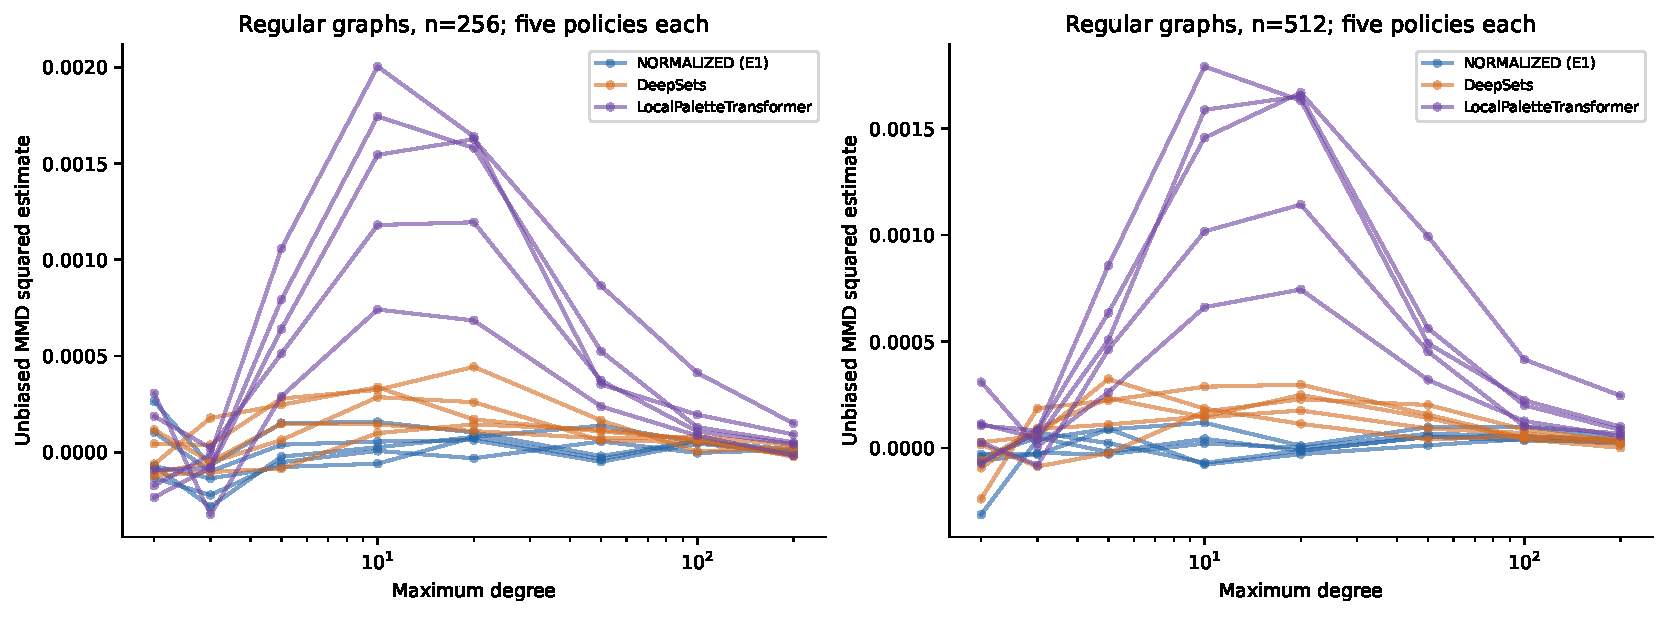
\includegraphics[width=\linewidth]{figures/global-degree.pdf}
\caption{Complete-vector unbiased MMD-squared estimates on the two fixed-size regular grids.
Each curve is one frozen training checkpoint; unbiased estimates may be
negative. These effects are graph-specific;
the normalized Hamming kernel does not make different graph spaces universally
comparable. One graph per grid cell limits graph-seed generalization.}
\end{figure}

All per-graph, checkpoint, raw and Holm-adjusted $p$-values are archived in
\texttt{primary.csv} in the study results; the accompanying
\texttt{rejected.csv} identifies exactly the cells supporting rejection.
Five-policy plots retain training variability separately from within-policy
Monte Carlo uncertainty. Structural diagnostics describe color usage,
class sizes, degree-conditioned color frequencies, co-color probabilities
and induced partitions; none substitutes for the labeled-vector hypothesis.
Secondary classifiers use independent training, validation and test banks.
A separately prospective supplement measures population power on the
three-vertex path using twenty disjoint experiments at each sample size and
seed 41000 of each architecture; an additional 100/250 subgrid covers the
star and regular power graphs. Binomial intervals retain finite-trial
uncertainty. A known-law supplementary star alternative has global TV $99/199$ while
its kernel effect is attenuated by $1-e^{-1/201}$; its independent detection
trials document finite-power limitations despite characteristicness.
Separate resampling power curves over 100--2,000 observations use empirical banks
for three prespecified graphs and seed 41000. Their intervals are
conditional on those banks and omit uncertainty in their population laws;
they describe nominal, not Holm-adjusted, detection rates.

Nonrejection means insufficient evidence at this sample size and correction,
not equality. Conservative pointwise population-MMD intervals do not establish
approximate equivalence at the preregistered tolerance $0.02$. Rejection
supports different solution laws only for its specified graph and frozen
policy. No universal monotone degree trend, population effect over training
seeds or graph families, or universal learned termination theorem follows.
The preregistration, exact-law proof, complete negative results and reproducible
figure sources accompany this provisional section.
